\section{\Large PROBLEM SET 5}
\subsection{PROBLEM 1}
\textit{Gravity gradient torque (stability)}

\textit{a. Calculate the coefficients Ki of the moments of inertia which drive stability under gravity gradient. Compute and plot regions of stable and unstable motion similar to the picture below:}

The following equations show the relationships for gravity gradient stability in terms of moments of inertia. The first inequality holds true when the pitch is stable and the last two inequalites hold true when the roll and yaw are stable.

\begin{align*}
    k_N = \frac{I_T - I_R}{I_N}, \;\;\;\;\;
    k_T = \frac{I_N - I_R}{I_T}, \;\;\;\;\;
    k_R = \frac{I_N - I_T}{I_R} \\
    k_T > k_R, \;\;\;\;\;
    k_R k_T > 0, \;\;\;\;\;
    1 + 3 k_T + k_R k_T > 4 \sqrt{k_R k_T}
\end{align*}


We show the plot of stable and unstable motion under gravity gradient. When computing the coefficients using moments of inertia about the principal axes, we obtain the following plot. In this case, we investigate the stability for the satellite when it is rotated such that the spacecraft is oriented appropriately for SAR operations, that is, principal x-axis is anti-radial, principal y-axis is opposite of cross-track, and principal z-axis is opposite of along-track. However, this orientation is unstable, as shown below.

\begin{figure}[H]
\centering
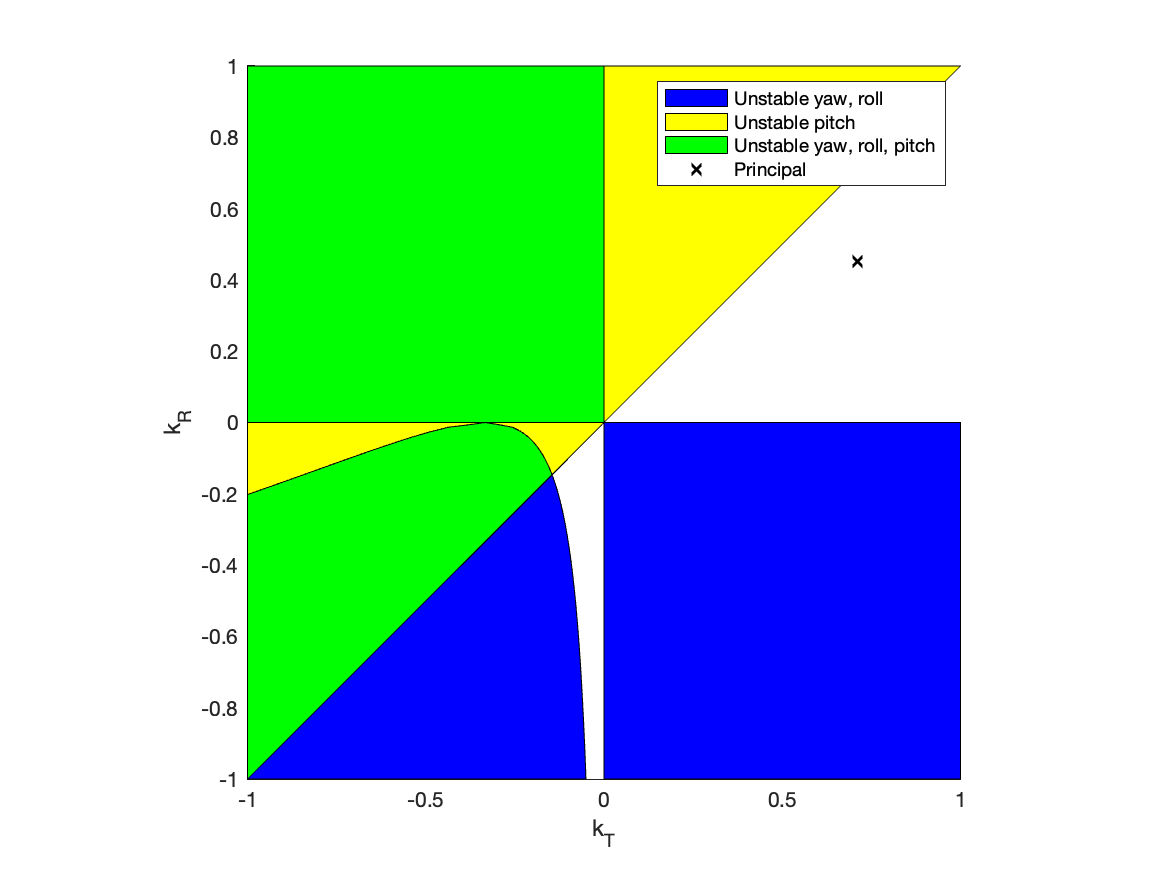
\includegraphics[scale=0.6]{Images/ps5_problem1a.png}
\caption{Stability for nominal axes}
\label{fig:ps5_problem1a}
\end{figure}

\textit{b. Considering the results from 1a, comments on the expected stability of the attitude motion of your satellite about equilibrium. Try to reproduce stable and unstable motion by setting proper initial conditions and perturbing those conditions slightly (e.g., by 1\%). Plot attitude parameters (e.g., Euler angles) to show stability or instability.}

First, without perturbations, the satellite can maintain steady attitude, demonstrating that this chosen orientation is indeed an equilibrium.

\begin{figure}[H]
\centering
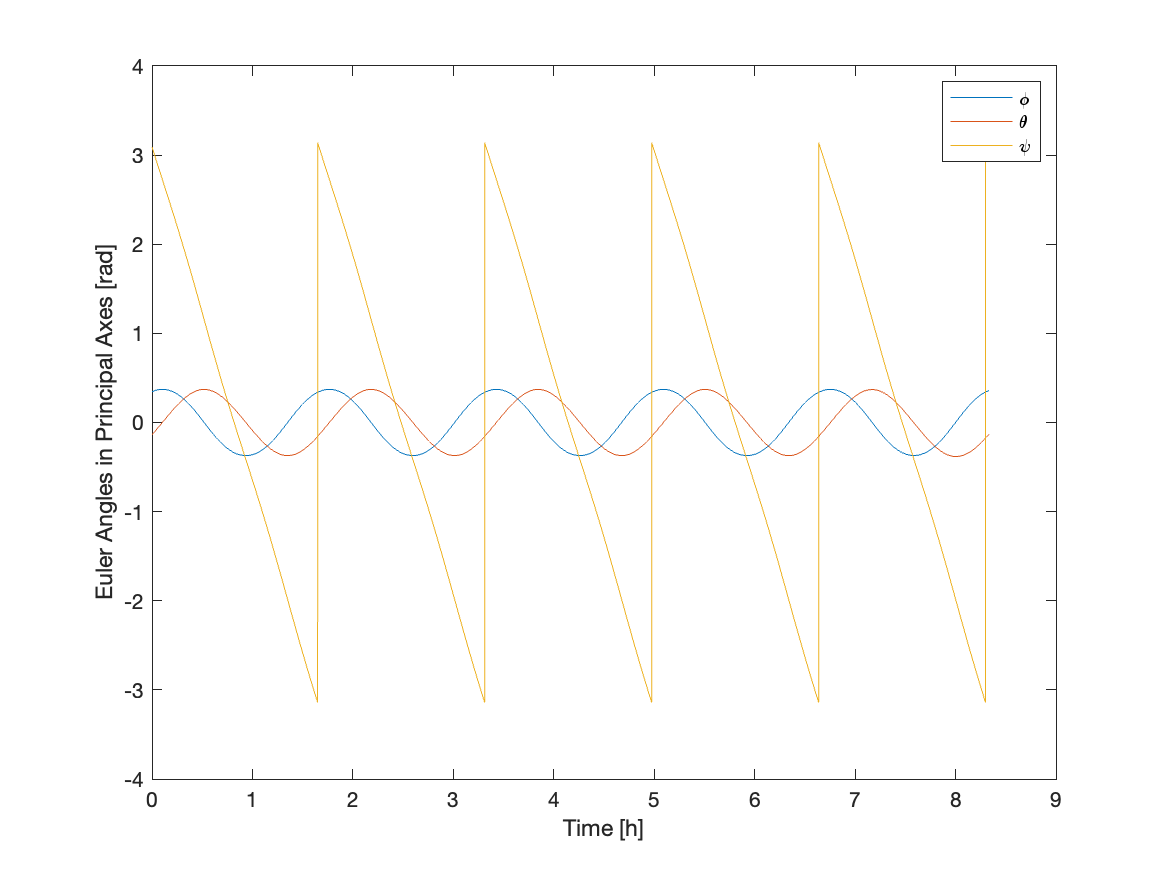
\includegraphics[scale=0.6]{Images/ps5_problem1b_angle_unperturbed.png}
\caption{Attitude evolution for unstable orientation without perturbations}
\label{fig:ps5_problem1b_angle_unperturbed}
\end{figure}

\begin{figure}[H]
\centering
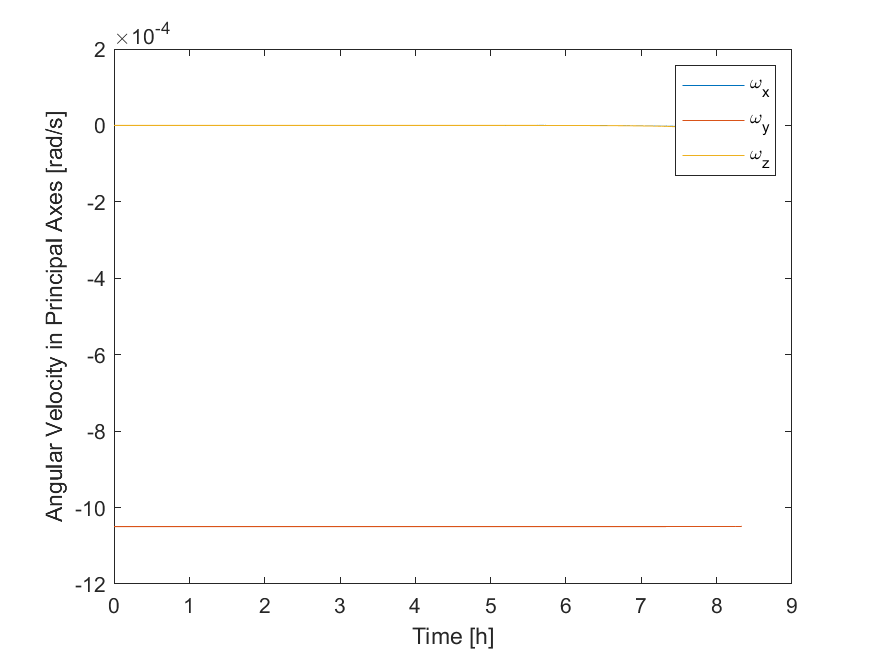
\includegraphics[scale=0.6]{Images/ps5_problem1b_angvel_unperturbed.png}
\caption{Angular velocity evolution for unstable orientation without perturbations}
\label{fig:ps5_problem1b_angvel_unperturbed}
\end{figure}

We expect unstable behavior for small perturbations. Previously, we have already shown that aligning principal axes with RTN produces stable behavior when there are no perturbations. Now, we will introduce small perturbations, causing the system to leave equilibrium and demonstrating that it is unstable.

\begin{figure}[H]
\centering
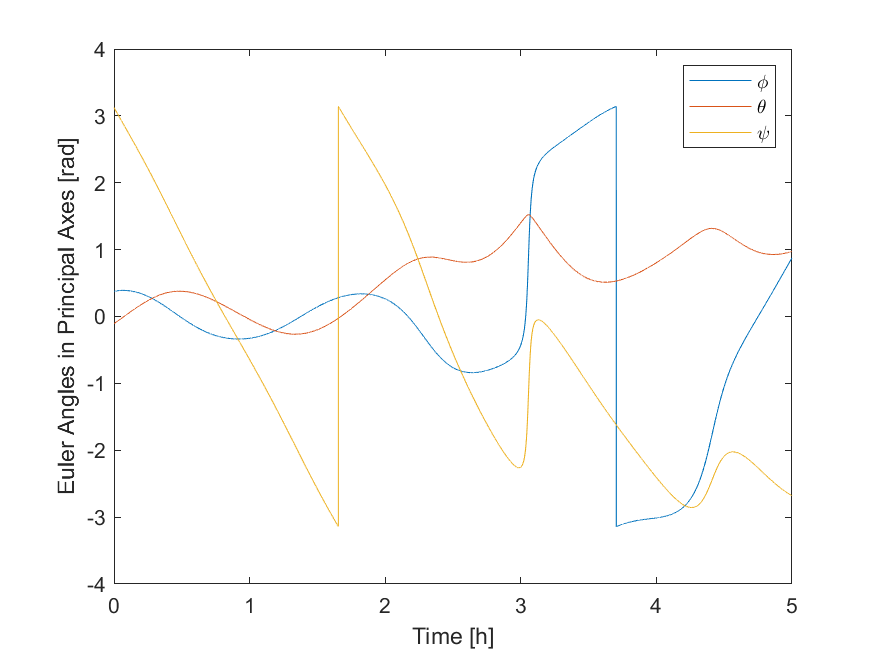
\includegraphics[scale=0.6]{Images/ps5_problem1b_angle.png}
\caption{Attitude evolution for unstable orientation with 1\% perturbations}
\label{fig:ps5_problem1b_angle}
\end{figure}

\begin{figure}[H]
\centering
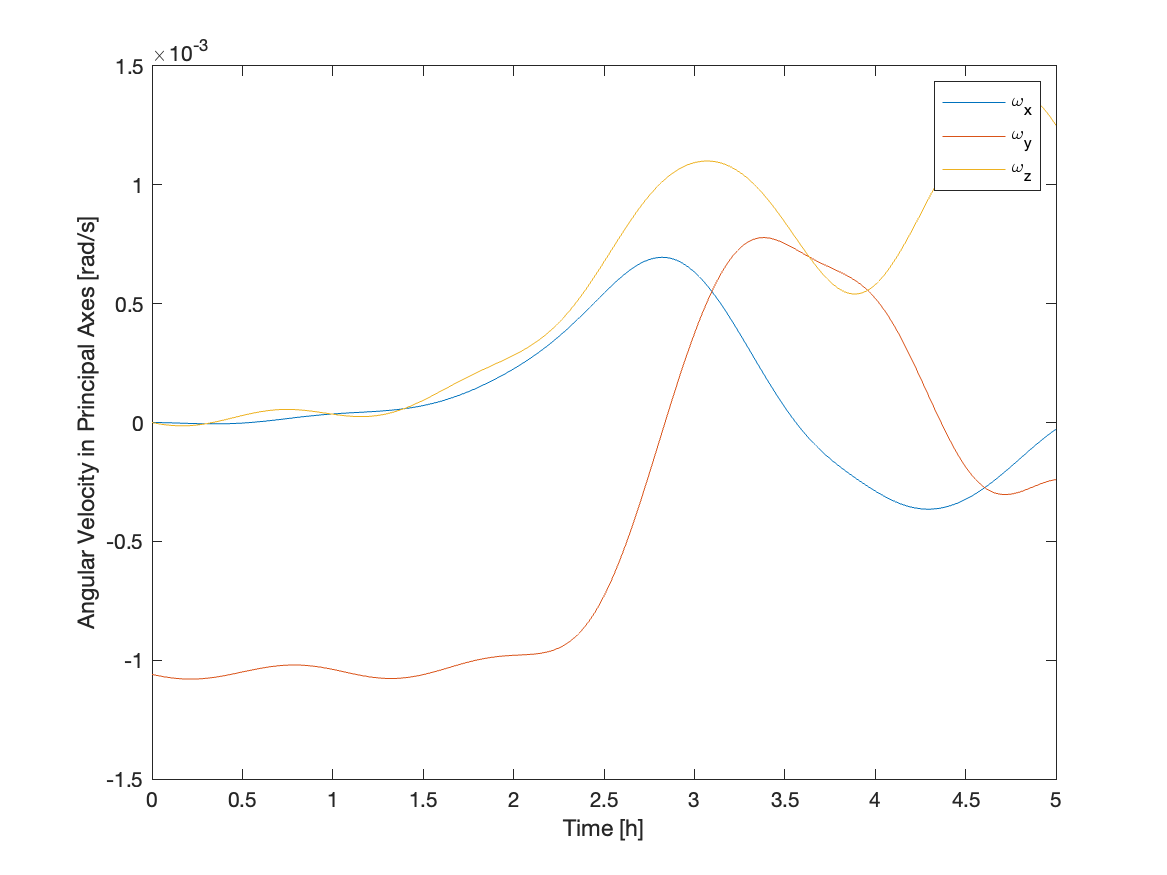
\includegraphics[scale=0.6]{Images/ps5_problem1b_angvel.png}
\caption{Angular velocity evolution for unstable orientation with 1\% perturbations}
\label{fig:ps5_problem1b_angvel}
\end{figure}


\textit{c. How would you need to change the mass distribution and/or nominal attitude of your satellite to obtain stable motion from the gravity gradient torque? Would it make sense for your project? Show a couple of potential configurations in the Ki plane and resulting stability of attitude motion at the equilibrium. This is done by changing your inertia tensor and simulating numerically.}

We will have to align the principal axes XYZ with RTN (respectively) to obtain a stable attitude motion.

\begin{figure}[H]
\centering
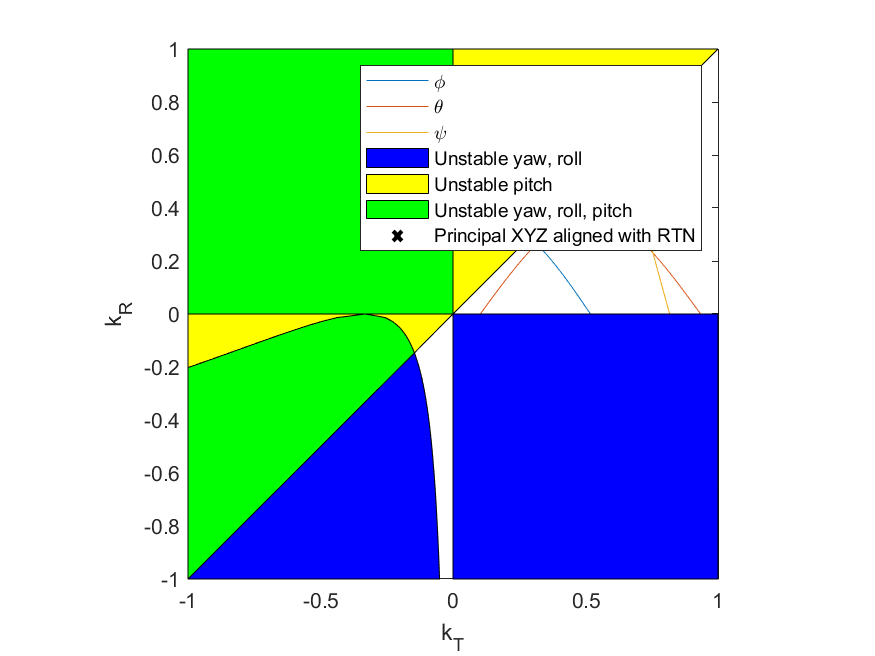
\includegraphics[scale=0.6]{Images/ps5_problem1c.png}
\caption{Stability for aligned principal axes}
\label{fig:ps5_problem1c}
\end{figure}

We expect stable behavior for small perturbations. Previously, we have already shown that aligning principal axes with RTN produces stable behavior when there are no perturbations. Now, we will introduce small perturbations.

\begin{figure}[H]
\centering
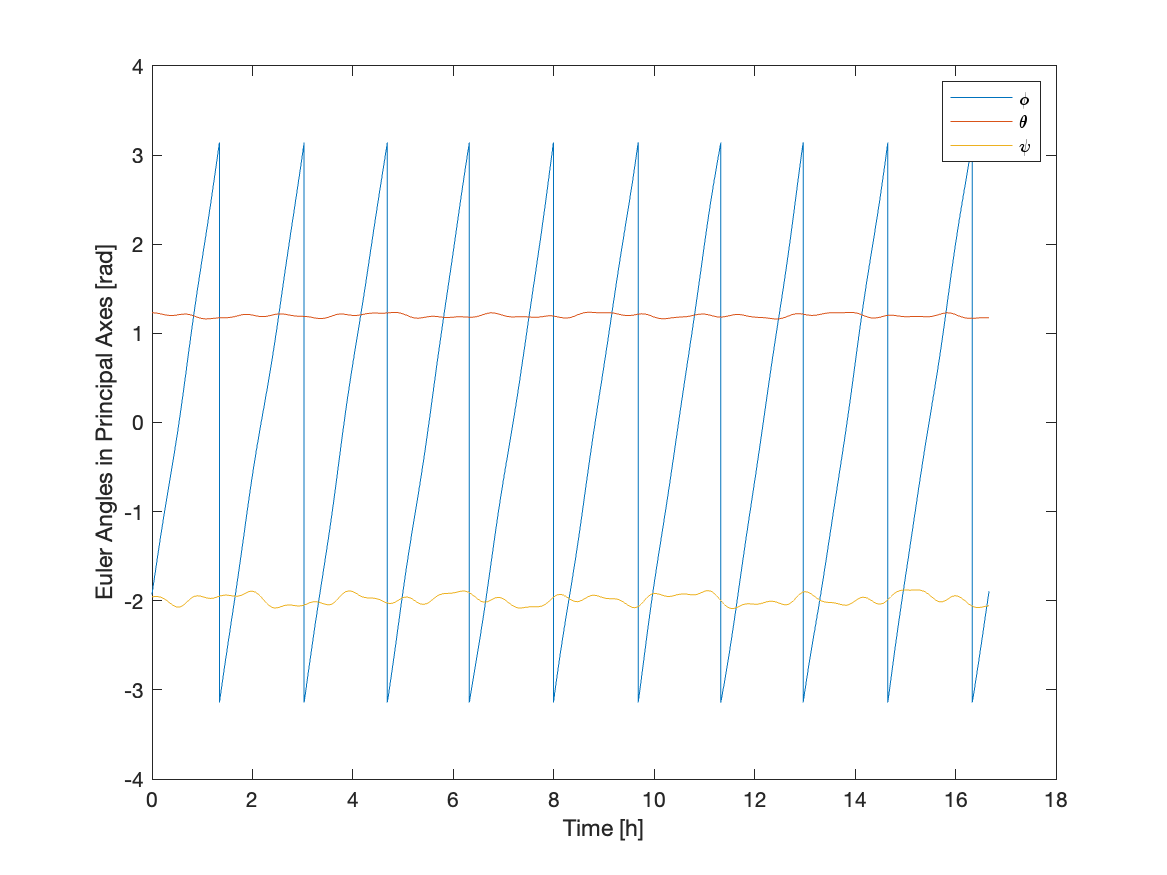
\includegraphics[scale=0.6]{Images/ps5_problem1c_angle.png}
\caption{Attitude evolution for stable orientation with 1\% perturbations}
\label{fig:ps5_problem1c_angle}
\end{figure}

\begin{figure}[H]
\centering
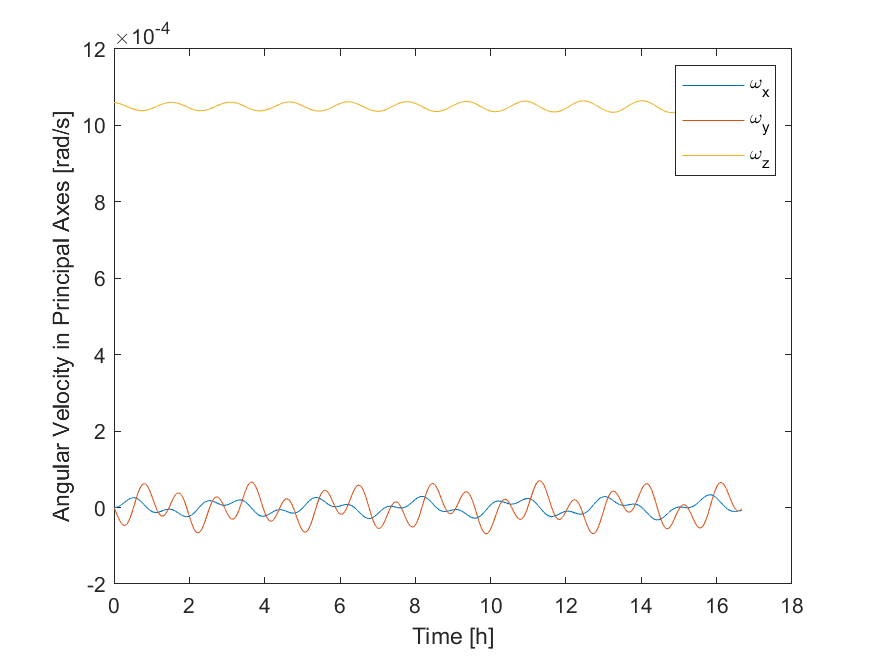
\includegraphics[scale=0.6]{Images/ps5_problem1c_angvel.png}
\caption{Angular velocity evolution for stable orientation with 1\% perturbations}
\label{fig:ps5_problem1c_angvel}
\end{figure}

As expected, our attitude motion (angular velocities and Euler angles) are periodically stable with a small perturbation in initial condition.

We cannot maintain this orientation if we want to properly point the radar antenna located at the top of the spacecraft, so it does not make sense to orient the satellite along principal axes for gravity gradient stability. Instead, we will likely require magnetorquers to offset angular momentum changes from environmental torques, including gravity gradient torques due to our unstable equilibrium.


\subsection{PROBLEM 2}
\textit{In addition to gravity gradient, start programming perturbation torques due to magnetic field, solar radiation pressure, and atmospheric drag. Note 1: You should apply a very minimal/basic model for perturbations that are not relevant (negligible) to your project. It is expected that you do not ignore them. Note 2: All perturbations can be grouped into a single large subsystem called environment or similar whose output feed
the Euler equations. Note 3: Re-use as many functions as possible for solar radiation pressure and atmospheric drag.}

In addition to gravity gradient torques, we modeled torque from magnetic field interactions, solar radiation pressure, and atmospheric drag.

The equation for the torque from the magnetic field interactions is below.

\begin{align*}
    \Vec{M}_{m} = \Vec{m}_{sat} \times \Vec{B}_{Earth}
\end{align*}

Since the satellite is expected operate in LEO, the spherical harmonic model up to n = 4 was used for maximum accuracy. This model is based on the geocentric distance ($R$), colatitude ($\theta$, and longitude $\phi$. The model requires Gaussian coefficients ($g^{n,m}$, $h^{n,m}$) and Legendre functions ($P^{n,m}$) and their derivatives ($\frac{\delta P^{n,m} (\theta)}{\delta \theta}$), which are explained in more detail in Wertz \cite{Wertz}.

\begin{align*}
    B_R = \sum^{4}_{n=1} (\frac{R_{Earth}}{R})^{n+2} (n+1) \sum^{n}_{m=0}
    (g^{n,m} \cos{m \phi} + h^{n,m} \sin{m \phi}) P^{n,m}(\theta) \\
    B_{\theta} = - \sum^{4}_{n=1} (\frac{R_{Earth}}{R})^{n+2} \sum^{n}_{m=0}
    (g^{n,m} \cos{m \phi} + h^{n,m} \sin{m \phi}) \frac{\delta P^{n,m} (\theta)}{\delta \theta} \\
    B_{\phi} = - \frac{1}{\sin{\theta}} \sum^{4}_{n=1} (\frac{R_{Earth}}{R})^{n+2}
    \sum^{n}_{m=0} m (-g^{n,m} \sin{m \phi} + h^{n,m} \cos{m \phi}) P^{n,m}(\theta)
\end{align*}

The equations below define the solar radiation torque, where $C_S$ is the specular reflection coefficient, $C_d$ is the diffuse reflection coefficient, $\Vec{S}$ is the vector facing the Sun, and $e_i$ is 1 if the surface is illuminated and 0 otherwise.

\begin{align*}
    \Vec{M}_{S} = \sum^{n}_{i=1} \Vec{r}_{i} \times e_i \int_{S_i} d \Vec{f}_{total_{i}} \\
    d \Vec{f}_{total} = -P ((1-C_S) \hat{\Vec{S}} + 2 (C_S \cos{\theta} + \frac{1}{3} C_d) \cos{\theta} dA
\end{align*}

The equations below define the aerodynamic torque.
\begin{align*}
    d \Vec{f}_{aero} = - \frac{1}{2} C_D \rho V^2 (\hat{\Vec{V}} \cdot \hat{\Vec{N}}) \hat{\Vec{V}} dA
\end{align*}


The following function enables the propagation of the orbit with the specified perturbation torques.

\lstinputlisting{src/orbitTorque.m}
\lstinputlisting{src/drag.m}
\lstinputlisting{src/srp.m}
\lstinputlisting{src/magFieldTorque.m}

\subsection{PROBLEM 3}
\textit{Include all torques you have been able to model in numerical integration. Please show comparison of numerically computed disturbance torques with expected values and trend from theory (model) and tables (Wertz) referenced in class. Plot all torque components in principal axes over time. Plot the resultant (sum) of all torques in principal axes. Make sure that your model is not too ideal, i.e. make sure that center of pressure and center of mass do not coincide.}

\begin{figure}[H]
\centering
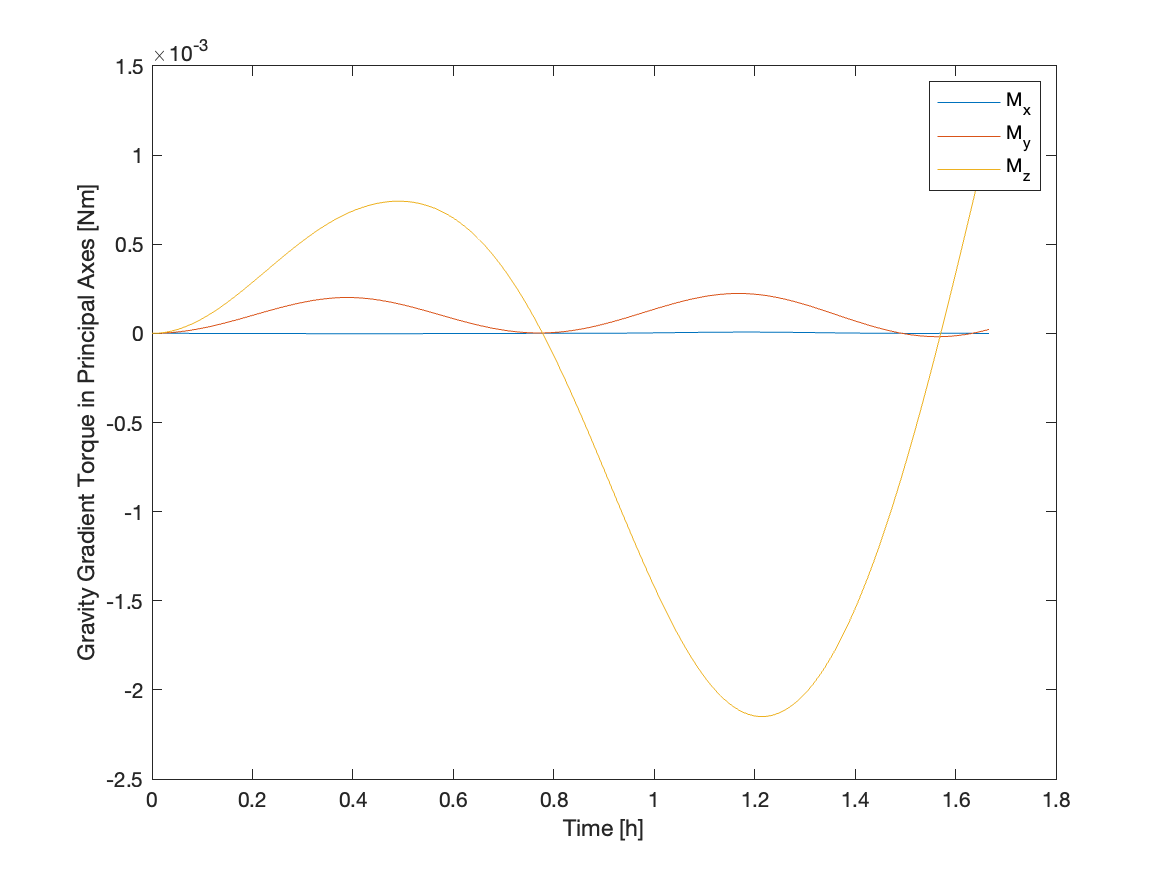
\includegraphics[scale=0.6]{Images/ps5_problem3_grav.png}
\caption{Numerical simulation of gravity gradient torques}
\label{fig:ps5_problem3_grav}
\end{figure}

\begin{figure}[H]
\centering
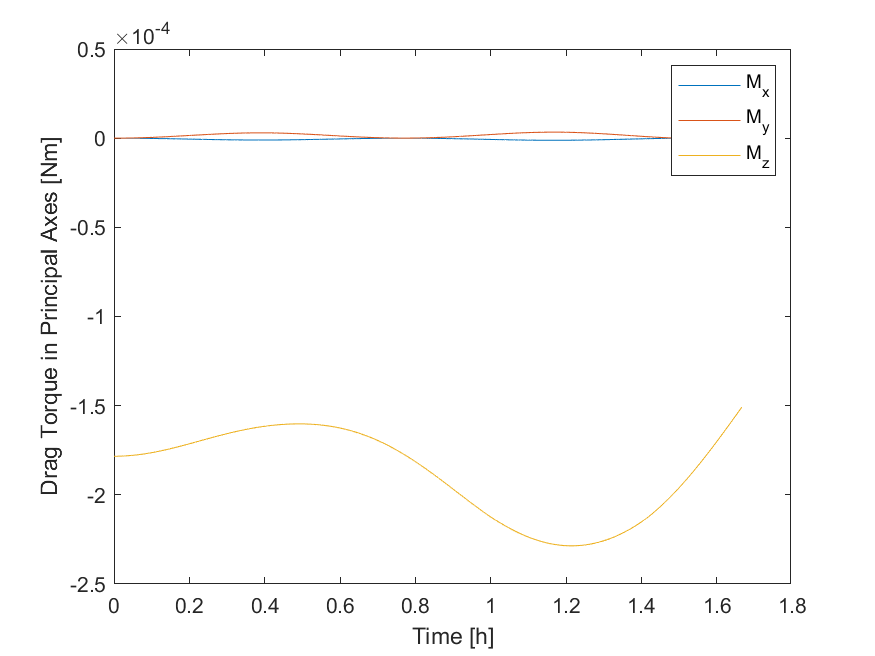
\includegraphics[scale=0.6]{Images/ps5_problem3_drag.png}
\caption{Numerical simulation of drag torques}
\label{fig:ps5_problem3_drag}
\end{figure}

\begin{figure}[H]
\centering
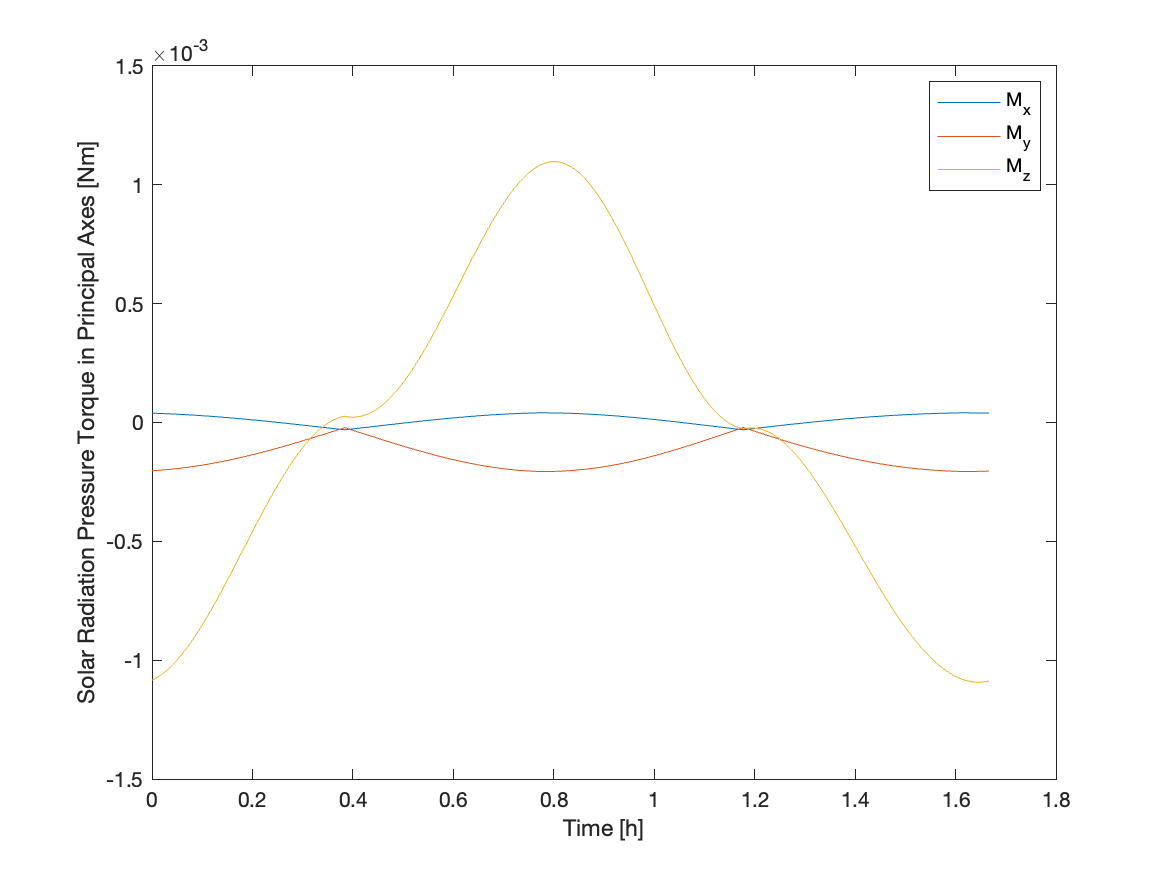
\includegraphics[scale=0.6]{Images/ps5_problem3_srp.png}
\caption{Numerical simulation of solar radiation pressure torques}
\label{fig:ps5_problem3_srp}
\end{figure}

\begin{figure}[H]
\centering
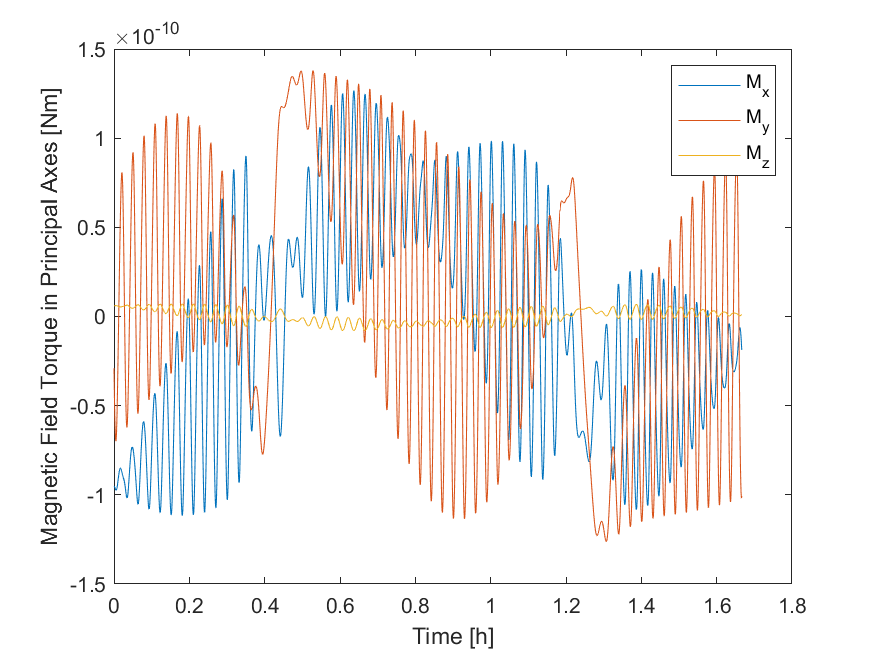
\includegraphics[scale=0.6]{Images/ps5_problem3_mag.png}
\caption{Numerical simulation of magnetic field torques}
\label{fig:ps5_problem3_mag}
\end{figure}